%
%		Este Modulo Explica como se registra la PQR
%
\section{Uso del Sistema de Gestión de PQRs}
\subsection {Tramite de una PQR}

\subsubsection{Estados de las PQR}

Antes de registrar las PQR, es importante tener en cuenta que éstas se clasifican por estados, 
el estado ayuda a conocer como va el trámite en el que se encuentra la PQR, de esta manera controlar su gestión.\\

Al crear la PQR el estado que se asigna es \textbf{nuevo}, si la PQR ya se encuentra en trámite
su estado será \textbf{en progreso}, si la PQR no se puede responder rápidamente, se puede pasar a un estado \textbf{pendiente} y si ya se le ha contestado al ciudadano, 
el estado es \textbf{cerrado}, una vez se cierra la PQR ésta no se puede modificar, y su reapertura está reservada para la persona que coordina el 
grupo de la oficina de atención al ciudadano.\\

El listado de PQRs pemite hacer filtros por estados tal como lo muestra la figura \ref{fig:menulista}

\begin{figure}[H]
 \centering
 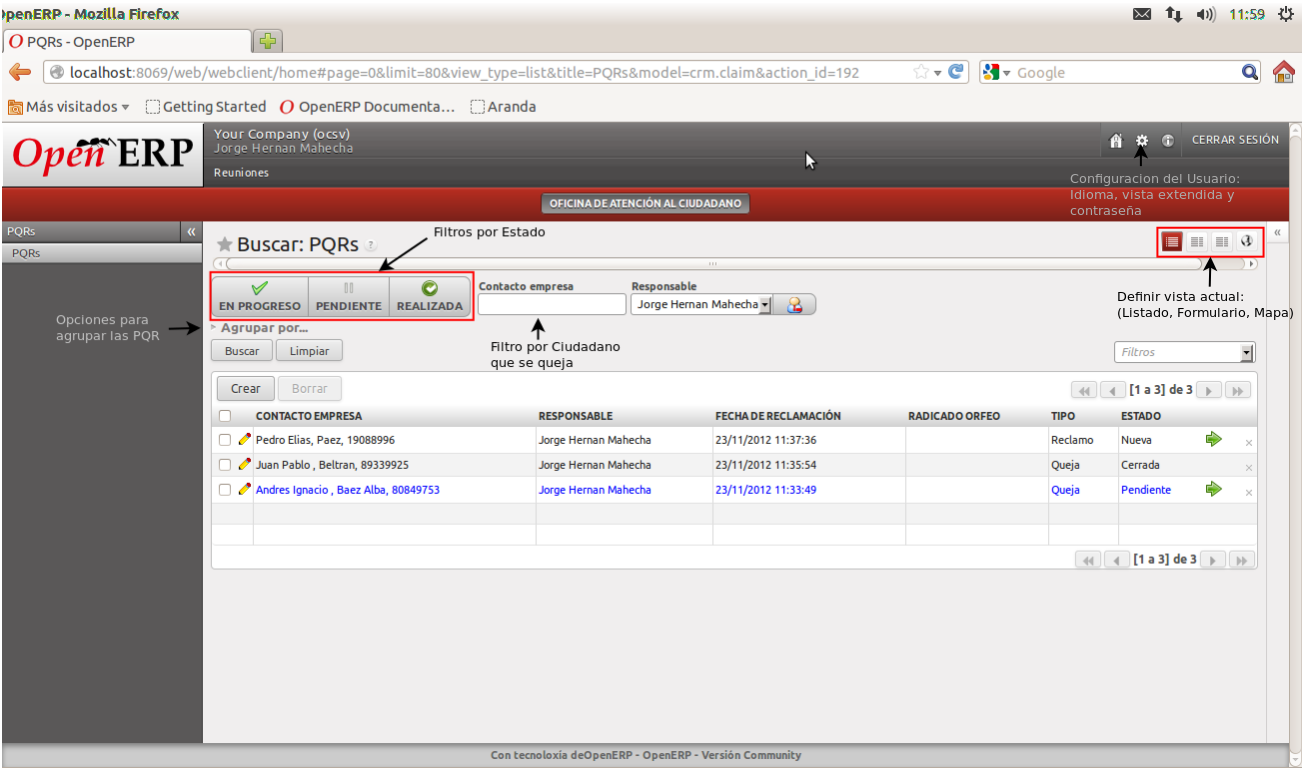
\includegraphics[width=17cm,height=10cm]{./Imagenes/menulista.png}
 % Login.png: 1289x610 pixel, 96dpi, 34.10x16.14 cm, bb=0 0 967 457
 \caption{Listado de PQR}
 \label{fig:menulista}
\end{figure}


\subsubsection{Creación de una PQR}

Para realizar el registro de una PQR se deben seguir los siguientes pasos:

\begin{itemize}
 \item Hacer clic en Oficina de Atención al Ciudadano $\Rightarrow$ PQR. 
 \item Hacer clic en el botón \textbf{Crear} que aparece en la grilla de la Lista, ver figura \ref{fig:menulista} 
 \item Aparecerá el formulario de la figura \ref{fig:formularioregistro}. Los datos que se deben ingresar son: El usuario que registra 
 la PQR (el usuario actual es seleccionado por defecto), el punto de atención donde se lleva a cabo dicha digitación (IDU, Cade), una prioridad, la fecha límite para tener la respuesta, el número
 de radicación en Orfeo si se tiene y el número de radicado de SDQS (Sistema Distrital de Quejas y Soluciones) si se tiene \footnote{En la actualidad 
 se está desarrollando el módulo para llevar a cabo dicho proceso automáticamente}. 
 \begin{figure}[H]
 \centering
 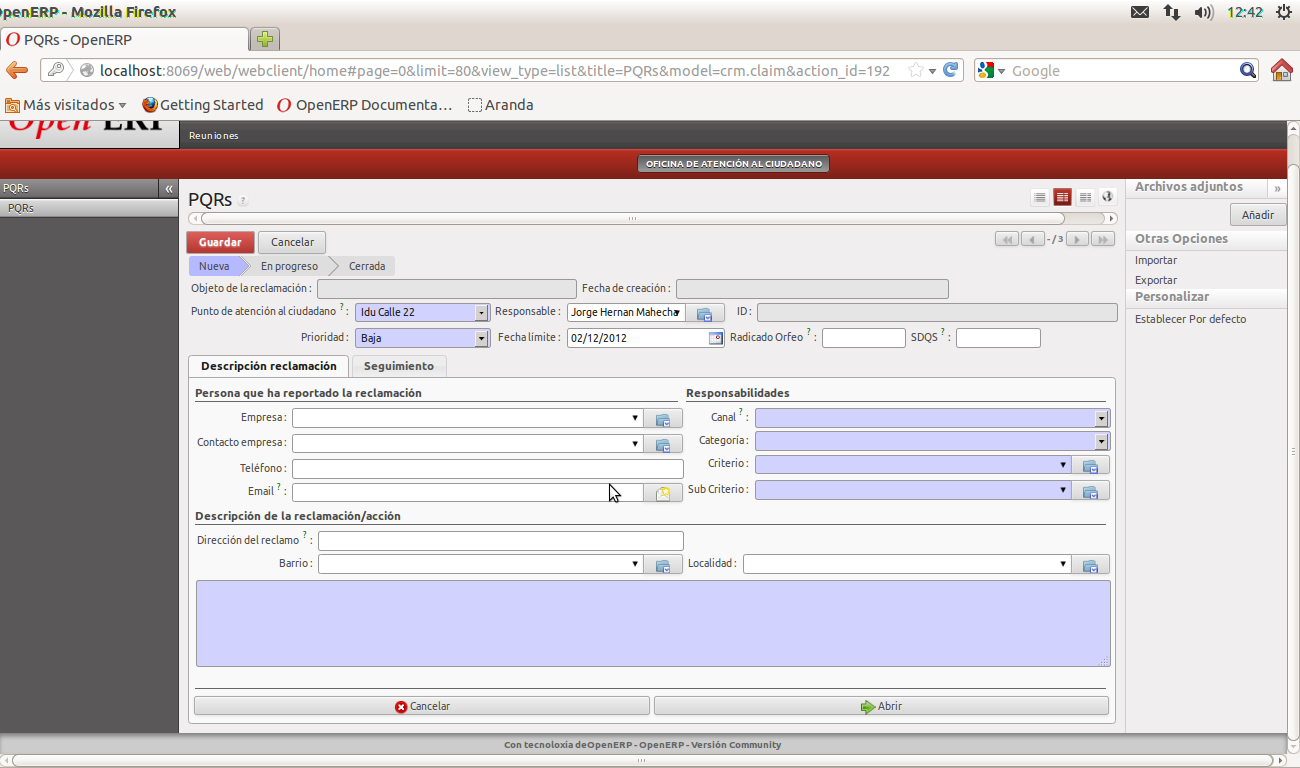
\includegraphics[width=17cm,height=10cm]{./Imagenes/formularioregistro.png}
 % Login.png: 1289x610 pixel, 96dpi, 34.10x16.14 cm, bb=0 0 967 457
 \caption{Formulario de registro de la PQR}
 \label{fig:formularioregistro}
\end{figure}

 \item En el campo para anotar los datos de la persona que hace la reclamación, se pueden presentar varios casos: 
 \begin{enumerate}
  \item La queja es anónima: en tal caso los campos donde se relacionan empresa y contacto van vacíos. 
  \item La queja es interpuesta por una empresa: se deben llenar los datos de ésta, y relacionar una persona de contacto. Para ello se deben llenar 
  los datos de la empresa, haciendo clic en el icono a la derecha del campo 
  \textbf{Empresa} , luego clic en \textbf{Crear}. Aparece una ventana emergente en donde se registran los
  datos básicos de la empresa (ver figura \ref{fig:pantempresa}), como lo es el nombre y el NIT (que se almacenará en el campo $CIF\backslash NIF$) 
  y \textbf{Guardar}. Se regresa a la pantalla anterior (figura \ref{fig:formularioregistro}. 
  En el campo contacto, se hace clic en el icono de la derecha y luego \textbf{Crear}. Aparecerá el formulario de la figura \ref{fig:formusuario}.
  En este formulario se ingresan los datos de la persona: Tipo de Documento, Numero de Documento, Primer Nombre, Segundo Nombre, la 
  empresa (Es la misma empresa que se acaba de ingresar), el cargo que desempeña en la empresa, y algún dato de contacto. Para que la 
  persona se pueda registrar, debe entregar al menos un dato de contacto.  Luego se hace clic en guardar.
  \begin{figure}[H]
  \centering
  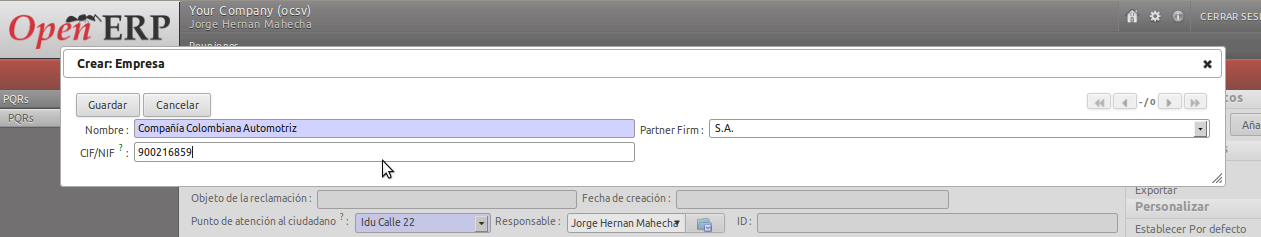
\includegraphics[width=17cm,height=4cm]{./Imagenes/pantempresa.png}
  % Login.png: 1289x610 pixel, 96dpi, 34.10x16.14 cm, bb=0 0 967 457
  \caption{Ventana emergente que solicita datos de la empresa}
  \label{fig:pantempresa}
  \end{figure}

  \begin{figure}[H]
  \centering
  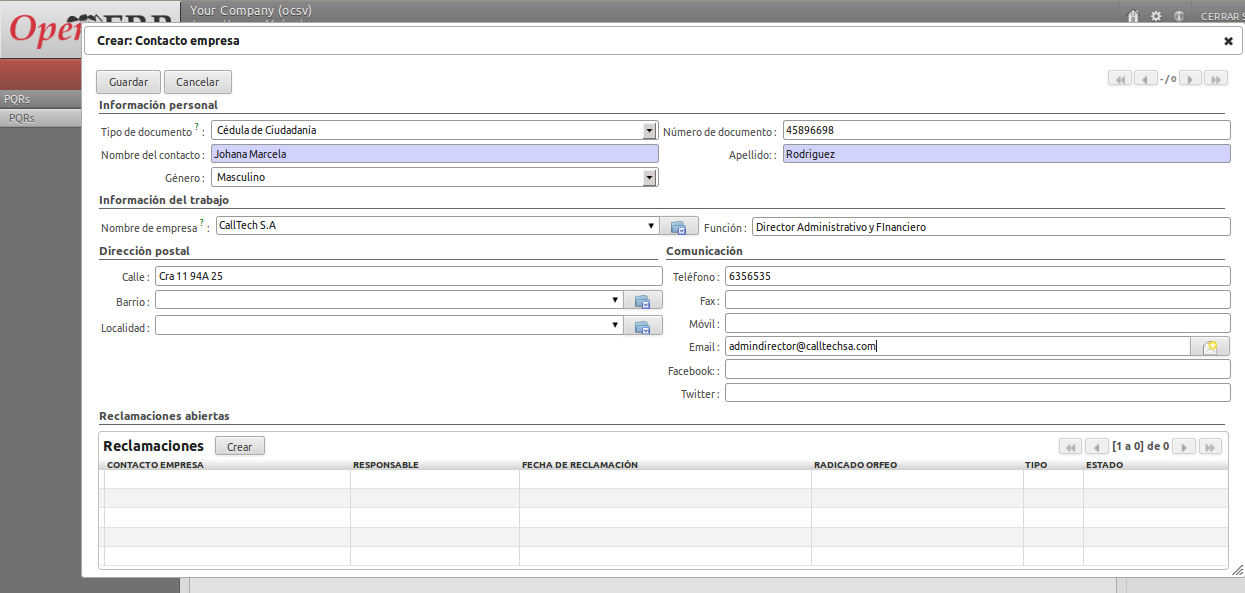
\includegraphics[width=17cm,height=8cm]{./Imagenes/formusuario.png}
  % Login.png: 1289x610 pixel, 96dpi, 34.10x16.14 cm, bb=0 0 967 457
  \caption{Ventana emergente para llenar la información de los ciudadanos}
  \label{fig:formusuario}
  \end{figure}

  \item La queja es interpuesta por una persona natural: Se ingresan los datos de la persona, para ello se hace clic en el icono a la izquierda  
  del campo contacto $\Rightarrow$ \textbf{Crear} y luego diligenciar el formulario de la figura \ref{fig:formusuario}.
 \end{enumerate}
 \item En el area señalada como responsabilidades, se selecciona el \textbf{Canal} por donde llegó la PQR, el \textbf{tipo de requerimiento},
 el \textbf{criterio} y \textbf{subcriterio} (\textbf{Tipificación}). Los subcriterios varían de acuerdo al criterio seleccionado, por tando es importante seleccionar
 primero el criterio, si no ve el criterio dentro las primeras opciones, puede ir escribiendo el texto hasta que aparezca en el cuadro el valor deseado, o 
 si no, simplemente hacer clic en el botón a la derecha y luego en \textbf{Buscar}. Allí se desplega un cuadro donde se puede seleccionar
 el criterio o subcriterio de una manera más cómoda (Ver figura \ref{fig:buscarcriterios}).
  \begin{figure}
  \centering
  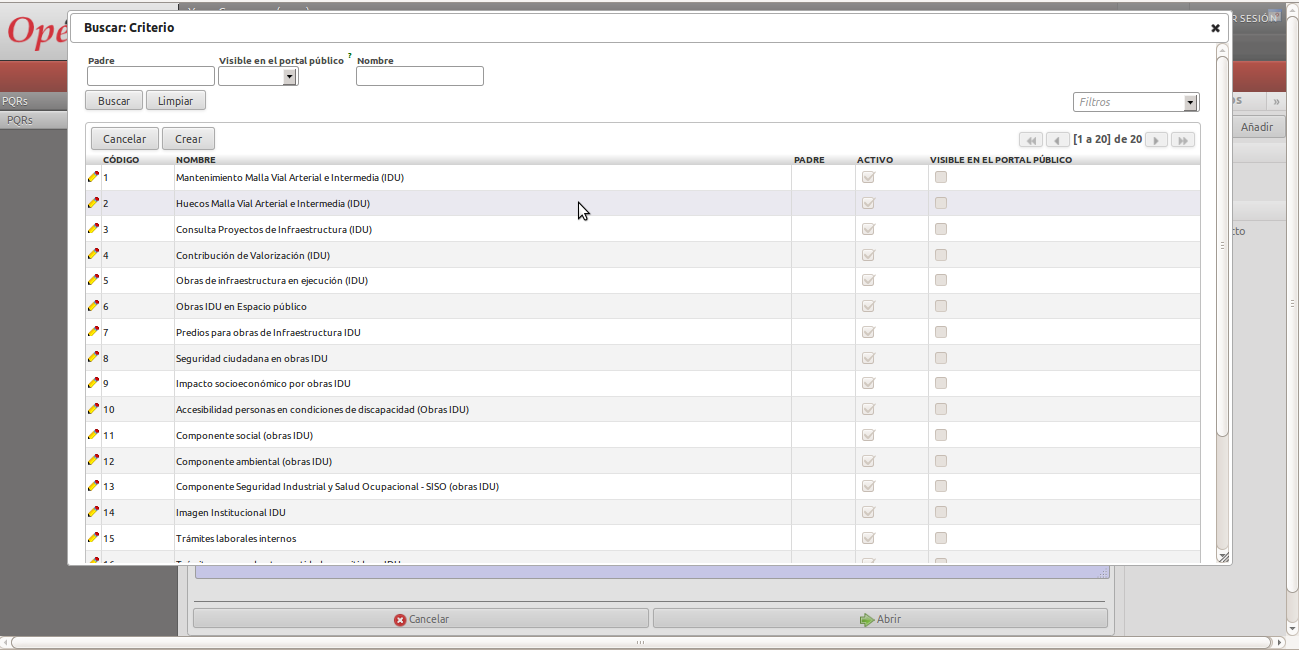
\includegraphics[width=17cm,height=10cm]{./Imagenes/buscarcriterios.png}
  % Login.png: 1289x610 pixel, 96dpi, 34.10x16.14 cm, bb=0 0 967 457
  \caption{Ventana emergente para buscar criterios y subcriterios}
  \label{fig:buscarcriterios}
  \end{figure}
 
 
 \item Luego llenar los datos de contacto y los criterios, 
 se registra el sitio de la reclamación, la localidad y el barrio, junto con
 el texto de la reclamación y se hace clic en \textbf{Abrir}, en ese momento la reclamación pasa a estado \textbf{en progreso}.
\end{itemize}

\begin{itemize}
 \item Si no se tiene la respuesta de la PQR a la mano, es importante pasarla a estado pendiente, para ello se hace clic en el botón \textbf{Pendiente} 
que se encuentra en la parte inferior del formulario. 
\item Si la respuesta del caso está se puede obtener en primera instancia, escriba el texto de respuesta en el campo \textbf{Solución} 
que se encuentra en la pestaña \textbf{Seguimiento}. Luego haga clic en el boton \textbf{Realizada} 
que se encuentra en la parte inferior del formulario (figura \ref{fig:formseguimiento}).
\end{itemize}

\begin{figure}[H]
 \centering
 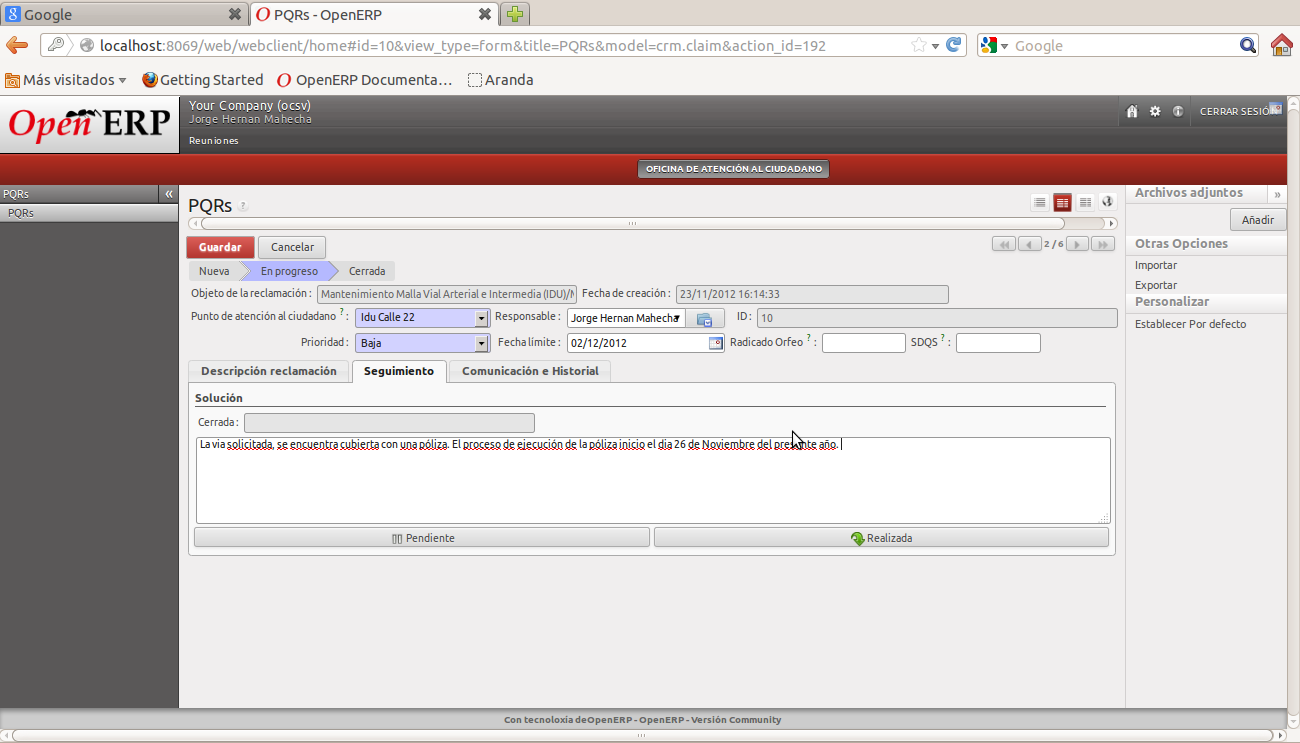
\includegraphics[width=17cm,height=10cm]{./Imagenes/formseguimiento.png}
 % Login.png: 1289x610 pixel, 96dpi, 34.10x16.14 cm, bb=0 0 967 457
 \caption{Formulario de la PQR con el campo para escribir el texto de solución}
 \label{fig:formseguimiento}
\end{figure}


\subsubsection{Cierre de la reclamación}


Siga los siguientes pasos para dar respuesta a la PQR:

\begin{itemize}
 \item Hacer clic en \textbf{Oficina de Atención al Ciudadano} $\Rightarrow$ PQR.
 \item En la lista (figura \ref{fig:menulista}) seleccionar el caso respectivo.
 \item Hacer clic en la pestaña \textbf{Seguimiento} y escribir la respuesta en el campo \textbf{Solución}.
 \item Hacer clic en el botón \textbf{Realizada} que se encuentra en la parte inferior del formulario. 
\end{itemize}

\subsection{Agregar Notas a una PQR}


Se pueden agregar anotaciones a la PQR, así com visualizar el historial de las acciones realizadas. Para hacerlo se debe habilitar
la interfaz web en modo extendido: 

\begin{itemize}
 \item Tomando como referencia la figura \ref{fig:menulista} hacer clic en el icono en forma de rueda que se encuentra a la
 izquierda del botón \textbf{CERRAR SESION}.
 \item Aparece un menú emergente de con las preferencias sobre el sistema (figura \ref{fig:configuracion}). En la opcion
  \textbf{Interfaz} seleccionar la opción \textbf{Extendida}. 
\begin{figure}[H]
 \centering
 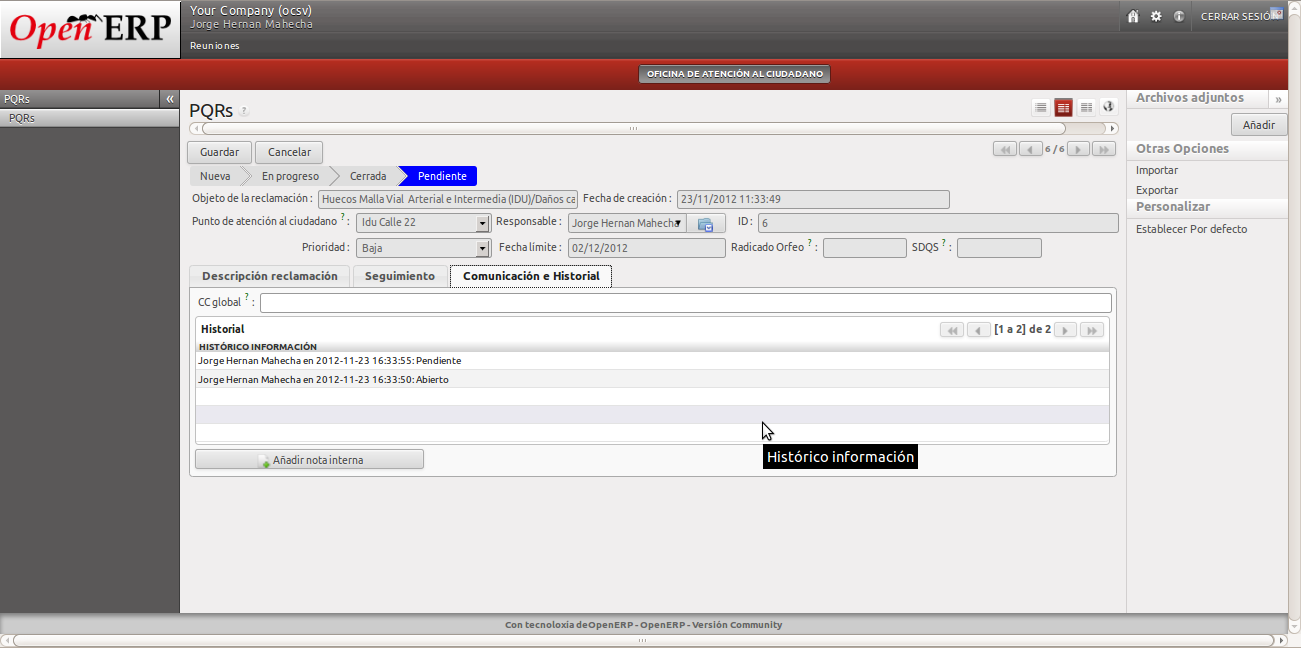
\includegraphics[width=17cm,height=10cm]{./Imagenes/historico.png}
 % Login.png: 1289x610 pixel, 96dpi, 34.10x16.14 cm, bb=0 0 967 457
 \caption{Historico de Acciones en la PQR}
 \label{fig:historico}
\end{figure}

 \item Este cambio hace que en general la aplicación muestre más opciones que cuando esta en modo simplificado. Al hacer 
 clic en \textbf{Oficina de Atención al Ciudadano} $\Rightarrow$ PQR $\Rightarrow$ Clic un caso cualquiera, se puede ver
 que en el formulario de la figura \ref{fig:formularioregistro} aparece la pestaña \textbf{Comunicación e Historial} 
 (figura \ref{fig:historico}). 
 \item Para agregar una nota se debe hacer clic en el botón \textbf{Añadir nota interna}, que aparece sobre la grilla.
 \item Se desplega la ventana ventana emergente de la figura \ref{fig:addnote}. Para añadir la nota se agrega el texto
 texto deseado y luego \textbf{Añadir}. 
\end{itemize}

\begin{figure}[H]
 \centering
 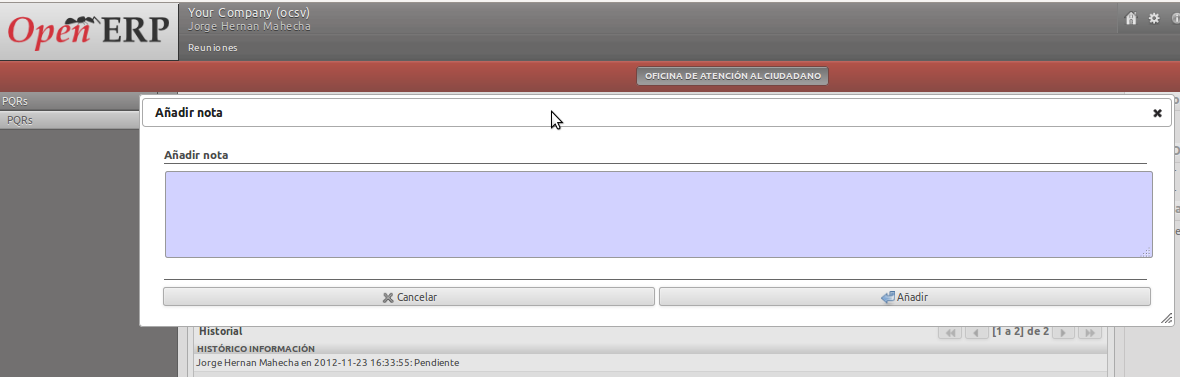
\includegraphics[width=17cm,height=6cm]{./Imagenes/addnote.png}
 % Login.png: 1289x610 pixel, 96dpi, 34.10x16.14 cm, bb=0 0 967 457
 \caption{Ventana Emergente para agregar notas internas}
 \label{fig:addnote}
\end{figure}

\subsection{Uso de la Vista de PQR en modo Lista}

Cuando se está en la vista de PQR en modo lista, se tienen algunas funcionalidades que ayudan a realizar un filtrado rápido de las mismas,
así como funciones de agrupación. 

Para agrupar las PQR hacer clic en el texto \textbf{Agrupar por}, de esta manera puede elegir los siguientes
criterios de agrupación (ver figura \ref{fig:menulistagroup}).
\begin{itemize}
 \item Responsable (Usuario a cargo de la PQR)
 \item Tipo (Petición, Queja, Reclamo, Sugerencia)
 \item Estado (Nuevo, Pendiente, En Progresso, Cerrado)
 \item Fecha de la Reclamación
 \item Fecha Limite
 \item Fecha de Cierre
\end{itemize}
\begin{figure}[H]
 \centering
 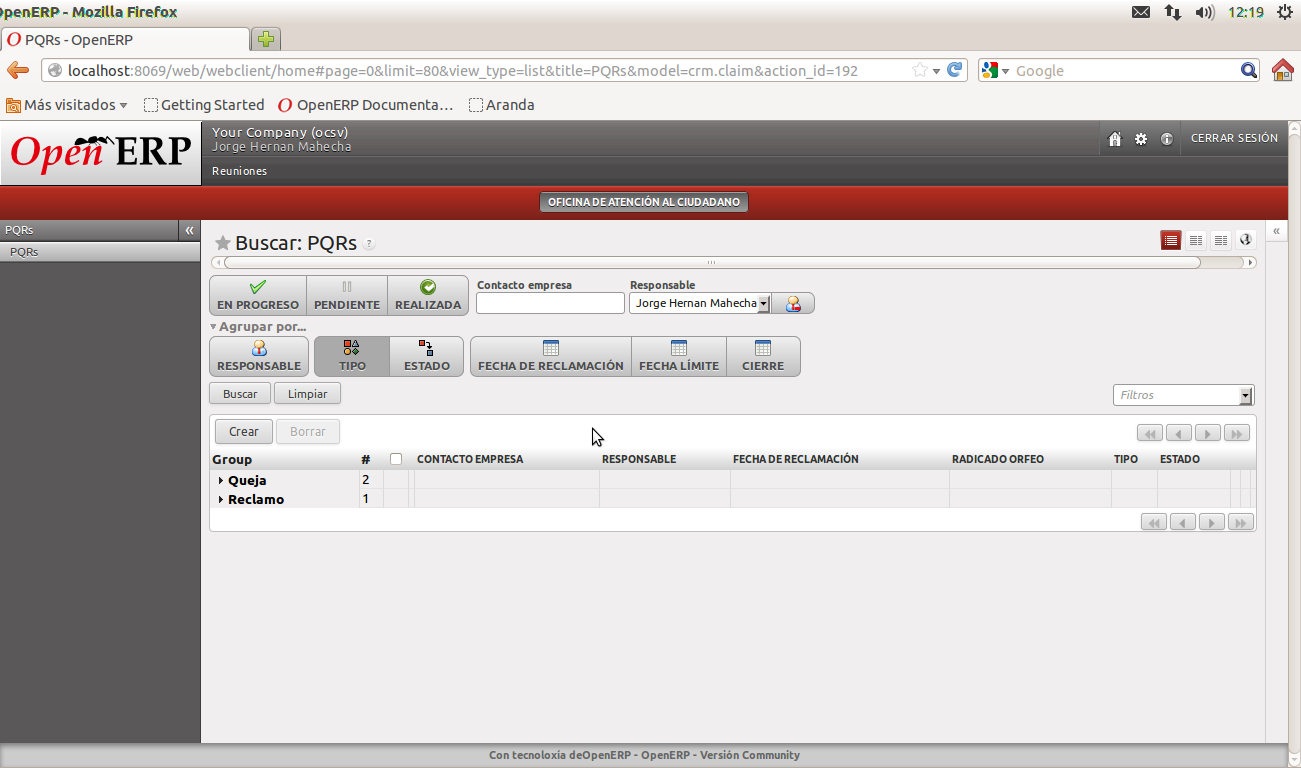
\includegraphics[width=17cm,height=10cm]{./Imagenes/menulistagroup.png}
 % Login.png: 1289x610 pixel, 96dpi, 34.10x16.14 cm, bb=0 0 967 457
 \caption{Agrupando la lista de PQR}
 \label{fig:menulistagroup}
\end{figure}

